\documentclass[a4paper,11pt]{article}

%%%%%%%%%%%%%%%%%%%%%%%%%%%%%%%%%%%%%%%%%%%%%%%%%%%%%%%%%%%%%%%%%%%%%%%%
% Paquetes utilizados
%%%%%%%%%%%%%%%%%%%%%%%%%%%%%%%%%%%%%%%%%%%%%%%%%%%%%%%%%%%%%%%%%%%%%%%%

% Gráficos complejos
\usepackage{graphicx}
\usepackage{subfig}
\usepackage{placeins}

% Soporte para el lenguaje español
\usepackage{textcomp}
\usepackage[utf8]{inputenc}
\usepackage[T1]{fontenc}
\DeclareUnicodeCharacter{B0}{\textdegree}
\usepackage[spanish]{babel}

% Código fuente embebido
\usepackage{listings}

% PDFs embebidos para el apéndice
\usepackage{pdfpages}

%%%%%%%%%%%%%%%%%%%%%%%%%%%%%%%%%%%%%%%%%%%%%%%%%%%%%%%%%%%%%%%%%%%%%%%%
% Título
%%%%%%%%%%%%%%%%%%%%%%%%%%%%%%%%%%%%%%%%%%%%%%%%%%%%%%%%%%%%%%%%%%%%%%%%

% Título principal del documento.
\title{\textbf{Trabajo Práctico 0: Infraestructura básica}}

% Información sobre los autores.
\author{
  Andrés Gastón Arana, \textit{P. 86.203}                          \\
  \texttt{and2arana@gmail.com}                                     \\
  Sergio Matías Piano, \textit{P. ??.???}                          \\
  \texttt{smpiano@gmail.com}                                       \\ [2.5ex]
  \normalsize{Grupo Nro. ? - 2do. Cuatrimestre de 2012}            \\
  \normalsize{66.20 Organización de Computadoras}                  \\
  \normalsize{Facultad de Ingeniería, Universidad de Buenos Aires}
}
\date{}

%%%%%%%%%%%%%%%%%%%%%%%%%%%%%%%%%%%%%%%%%%%%%%%%%%%%%%%%%%%%%%%%%%%%%%%%
% Documento
%%%%%%%%%%%%%%%%%%%%%%%%%%%%%%%%%%%%%%%%%%%%%%%%%%%%%%%%%%%%%%%%%%%%%%%%

\begin{document}

\thispagestyle{empty}
\maketitle

\begin{abstract}
  Este informe sumariza el desarrollo del trabajo práctico 0 de la materia
  Organización de Computadoras (66.20) dictada en el segundo cuatrimestre de
  2012 en la Facultad de Ingeniería de la Universidad de Buenos Aires. El mismo
  consiste en la construcción de un sistema minimalista de ordenamiento de
  archivos y el análisis de performance y perfilado del mismo, con foco en la
  generación de un entorno de infraestructura básica para soportar el
  desarrollo de estas tareas que será reutilizado en futuros trabajos
  prácticos.
\end{abstract}

\clearpage

\tableofcontents
\clearpage

\part{Desarrollo}
\section{Introducción}

TODO: Definir

\section{Desarrollo}

\section{Conclusiones}

TODO: Definir

\begin{thebibliography}{99}

\bibitem{INT06} Intel Technology \& Research, ``Hyper-Threading Technology,'' 2006, http://www.intel.com/technology/hyperthread/.

\end{thebibliography}

\clearpage
\part{Apéndice}
\appendix
\section{README del material digital}

\includepdf[pages={-}]{build/doc/README.pdf}

\section{Código fuente}
\clearpage
\definecolor{gray}{rgb}{0.5,0.5,0.5}
\lstset{
  language=C,
  title=\lstname,
  basicstyle=\footnotesize,
  showspaces=false,
  showstringspaces=false,
  breaklines=true,
  commentstyle=\color{gray},
  numbers=left,
  numberstyle=\tiny\color{gray},
  numbersep=5pt,
}

\lstinputlisting{source/buffer.h}
\lstinputlisting{source/buffer.c}
\lstinputlisting{source/clargs.h}
\lstinputlisting{source/clargs.c}
\lstinputlisting{source/cltext.h}
\lstinputlisting{source/cltext.c}
\lstinputlisting{source/config.h}
\lstinputlisting{source/data.h}
\lstinputlisting{source/data.c}
\lstinputlisting{source/quicksort.h}
\lstinputlisting{source/quicksort.c}
\lstinputlisting{source/stooge.h}
\lstinputlisting{source/stooge.c}
\lstinputlisting{source/tp0.c}


\section{Enunciado original}

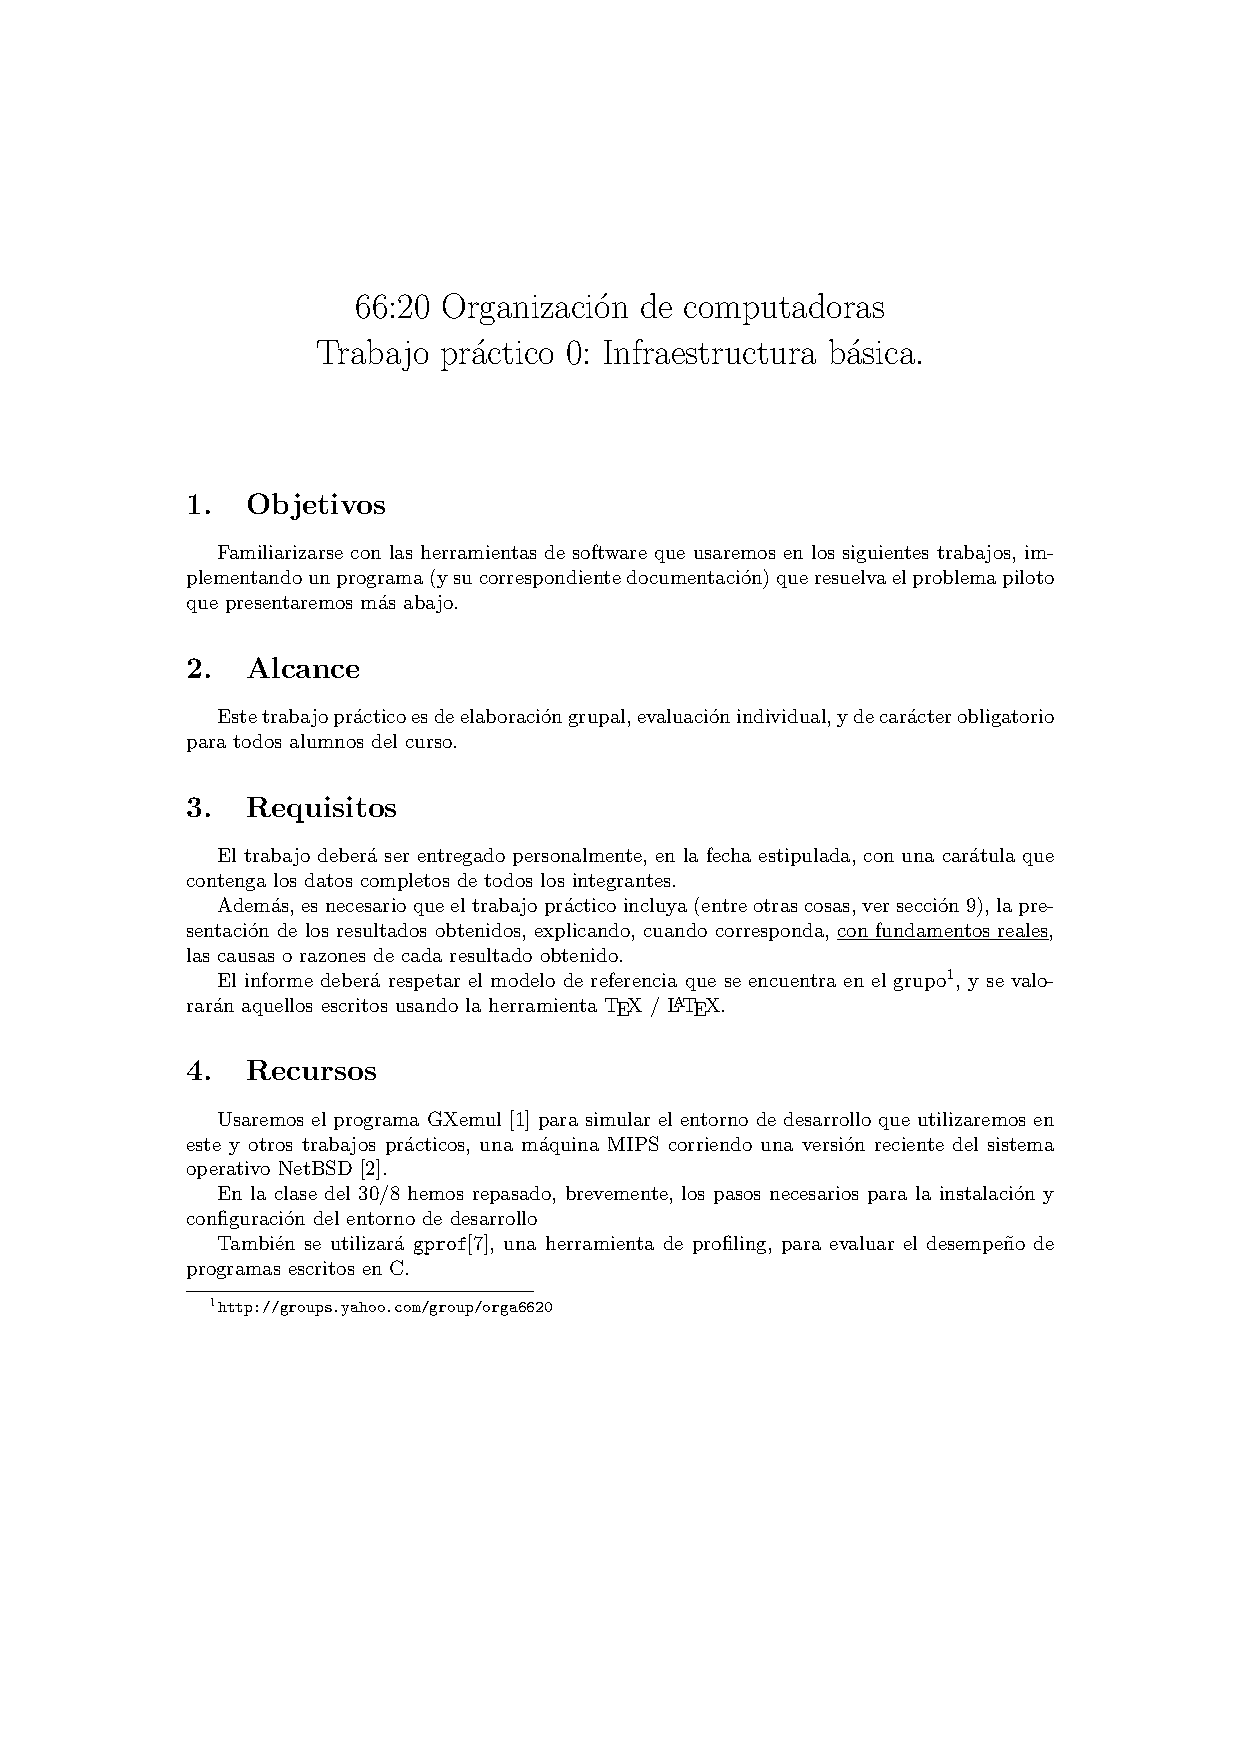
\includepdf[pages={-}]{docs/enunciado.pdf}

\end{document}
